\documentclass[letterpaper,10pt]{article}

\usepackage{titling}
\usepackage{listings}
\usepackage{url}
\usepackage{setspace}
\usepackage{subfig}
\usepackage{sectsty}
\usepackage{pdfpages}
\usepackage{colortbl}
\usepackage{multirow}
\usepackage{relsize}
\usepackage{amsmath}
\usepackage{fancyvrb}
\usepackage{amsmath,amssymb,amsthm,graphicx,xspace}
\usepackage[titlenotnumbered,noend,noline]{algorithm2e}
\usepackage[compact]{titlesec}
\usepackage[default]{droidserif}
\usepackage[T1]{fontenc}
\usepackage{tikz}
\usetikzlibrary{arrows,automata,shapes,trees,matrix,chains,scopes,positioning,calc}
\tikzstyle{block} = [rectangle, draw, fill=blue!20, 
    text width=2.5em, text centered, rounded corners, minimum height=2em]
\tikzstyle{bw} = [rectangle, draw, fill=blue!20, 
    text width=4em, text centered, rounded corners, minimum height=2em]

\definecolor{namerow}{cmyk}{.40,.40,.40,.40}
\definecolor{namecol}{cmyk}{.40,.40,.40,.40}

\let\LaTeXtitle\title
\renewcommand{\title}[1]{\LaTeXtitle{\textsf{#1}}}


\newcommand{\handout}[5]{
  \noindent
  \begin{center}
  \framebox{
    \vbox{
      \hbox to 5.78in { {\bf ECE155: Engineering Design with Embedded Systems } \hfill #2 }
      \vspace{4mm}
      \hbox to 5.78in { {\Large \hfill #4  \hfill} }
      \vspace{2mm}
      \hbox to 5.78in { {\em #3 \hfill} }
    }
  }
  \end{center}
  \vspace*{4mm}
}

\newcommand{\lecture}[3]{\handout{#1}{#2}{#3}{Lecture #1}}
\newcommand{\tuple}[1]{\ensuremath{\left\langle #1 \right\rangle}\xspace}

\addtolength{\oddsidemargin}{-1.000in}
\addtolength{\evensidemargin}{-0.500in}
\addtolength{\textwidth}{2.0in}
\addtolength{\topmargin}{-1.000in}
\addtolength{\textheight}{1.75in}
\addtolength{\parskip}{\baselineskip}
\setlength{\parindent}{0in}
\renewcommand{\baselinestretch}{1.5}
\newcommand{\term}{Spring 2014}

\singlespace


\begin{document}

\lecture{ 18 --- Software Requirements \& Specifications}{\term}{Jeff Zarnett}

\section*{About Software Requirements}

A \textit{Software Requirement} is, simply put, something that a piece of software is expected to do. It describes what the software should do, but not how the software should do it. Requirements can be formal in the sense of long, written documents or they can be informal.

\paragraph{Why Bother?} Software requirements maybe seem like a lot of overhead and planning and maybe it doesn't seem like a very XP activity. But it is necessary to have some goals, no matter what methodology you are using. Without requirements (however informal), how do you know what to do? How do you know the software meets its goals if you don't have clearly defined goals?

A \textit{Functional Requirement} is a something the system does - a function or task. Imagine we are making a piece of software for the university so student grades can be entered quickly and easily. What are some examples of functional requirements?

\begin{itemize}
	\item Professors must be able to input grades.
	\item Professors must be able to update grades once entered.
	\item The system must compute class averages.
	\item Administrators must be able to search for a student's history.
\end{itemize}

A \textit{Non-Functional Requirement} is not something the software does, but it described the behaviour of the system. Let's look at some examples of non-functional requirements.

\begin{itemize}
	\item Professors should be easily able to learn the system.
	\item A student may not see the grades of other students.
	\item A record search must take less than five seconds.
	\item The system downtime must be less than eight hours per month.
\end{itemize}

And finally there are \textit{Constraints}, a specialized type of non-functional requirement that restricts the design or implementation of the system. For example:

\begin{itemize}
	\item The server must run on Linux.
	\item The database must be MySQL.
	\item The server must be implemented using C++.
\end{itemize}

Sometimes it is not clear whether a requirement is functional or non-functional. The important thing to remember is that a functional requirement is a task the software does, and a non-functional requirement is a quality of the system. Security, phrased broadly, is a non-functional requirement. However, the ability for administrators to lock a compromised account is a functional requirement. 

It's very common, when writing down requirements, to come up with a ``mixed'' requirement, that reads something like: ``The user must be able to search for music on his phone and see results within 10 seconds''. This might be fine in your document, but it is important to know that this encompasses a functional component (being able to search) and a non-functional component (results within 10s).

There is some further controversy on whether some software requirements are truly meaningful without associated non-functional requirements. If a system is designed to search songs on your phone, and the search takes one full week to complete, the functional requirement is technically satisfied, but the system is not very useful...

\subsection*{Stories}
Stories feature prominently in Behaviour-Driven Development, and it is the idea that we can describe requirements in a natural way so that the customer, developers, and testers understand the work that is to be done. If all parties have a common definition of done, then the situation of the customer saying ``that's not what I wanted'' is much less likely to occur. 

A story follows (roughly) this template \cite{bdd2}:

\begin{quote}
Title (one line describing the story)\\

Narrative:\\
As a [role]\\
I want [feature]\\
So that [benefit]\\

Acceptance Criteria: (presented as Scenarios)

Scenario 1: Title\\
Given [context]\\
  And [some more context]...\\
When  [event]\\
Then  [outcome]\\
  And [another outcome]...\\

Scenario 2: ...
\end{quote}

That title should give a summary of some behaviour of a user of the system. It is the first step in deciding what work is to be done. A vague title like ``Module X Behaviour'' does not lend itself to telling a focused, cohesive story; a title like ``User Prints an Invoice'' is much clearer.

The narrative includes: A role (who will interact with the system?), a feature (what to implement?), and a benefit (why do this?). The answers to these three questions provide most of the information about the story. The ``why'' of the story is especially important; if you have no answer (or a bad answer like ``because the old system did this''), then you may not have to implement this feature at all.

Finally, the scenarios at the bottom. The title should give an indication of what is different in the scenario (example: ``User does not have permission to print invoices'') followed by a brief description. A scenario description contains three elements: Given, When, and Then. The Given provides the set-up or context, the When describes the event that takes place, and the Then describes the outcome(s). 

One key question is how much detail needs to be provided at each section of the story. There is no hard rule, but enough detail is required that everyone has a complete understanding of the story. On the other hand, brevity is appreciated because nobody likes reading long, boring documents.

\paragraph{Example.} Here is the obligatory Automatic Teller Machine (ATM) example (every software requirements discussion must have one). It is presented in the form of a story (from \cite{bdd2}).

\begin{quote}
Story: Account Holder Withdraws Cash\\

As an Account Holder\\
I want to withdraw cash from an ATM\\
So that I can get money when the bank is closed

\textbf{Scenario 1: Account has sufficient funds}\\
Given the account balance is \$100\\
 And the card is valid\\
 And the machine contains enough money\\
When the Account Holder requests \$20\\
Then the ATM should dispense \$20\\
 And the account balance should be \$80\\
 And the card should be returned

\textbf{Scenario 2: Account has insufficient funds}\\
Given the account balance is \$10\\
 And the card is valid\\
 And the machine contains enough money\\
When the Account Holder requests \$20\\
Then the ATM should not dispense any money\\
 And the ATM should say there are insufficient funds\\
 And the account balance should be \$10\\
 And the card should be returned

\textbf{Scenario 3: Card has been disabled}\\
Given the card is disabled\\
When the Account Holder requests \$20\\
Then the ATM should retain the card\\
And the ATM should say the card has been retained

\textbf{Scenario 4: The ATM has insufficient funds}\\
...

\end{quote}

There is no upper limit to how many scenarios there might be in a story, but after a certain point it might make sense to break a story down into some smaller stories which are easier to comprehend and test. To do so, expand the list of assumptions to make the stories mutually exclusive, yet complete. Perhaps the previous example could be broken down into:

\begin{itemize}
	\item Account holder withdraws cash (assumptions: ATM is working, card is valid)
	\item Account holder attempts to withdraw cash from broken ATM (assumptions: ATM is malfunctioning, card is valid)
	\item Account holder attempts to withdraw cash with invalid card (assumptions: ATM is working, card is invalid)
\end{itemize}


\subsection*{Gathering Software Requirements}

Of course, software requirements come from somewhere. Typically, that means you have to create them. When you or your company wants to make a piece of software, often it is to meet the needs of a (potential) customer. We gather requirements as a way to get user and stakeholder input into the design of the system.

How do you gather software requirements, then? There is one very important way \textbf{not} to do it. You cannot let your customers dictate your requirements to you. The fact is that customers do not know what they want, and this goes double for customers who are non-technical. For the most part, users are unable to imagine anything other than a marginally better version of a system they have already worked with. Or, to put it more succinctly:

\begin{quote}
	\textit{If I had asked people what they wanted, they would have said faster horses.}
\end{quote}
\vspace{-1.5em}
\hfill Henry Ford (possibly).

If you ignore this, the likely outcome is that you will create a piece of software the the users will not accept or cannot use. This is not to say that user input is irrelevant, but it is only one piece of the puzzle. Some common techniques for soliciting user input are: (1) meeting with a focus group of users and asking them questions; (2) following users in their daily workflow; and (3) brainstorming.

Stories are generated, ideally, with the input of several people. A tester (programmer), business analyst, and the customer should be represented. It is an iterative process: the stakeholder suggests something they want, and the business analyst and tester turn that into a story. They show it to the customer, and the customer likely has more input: edge cases, more details, or even saying that the story is on the wrong track \cite{bdd2}.

Remember that what you get from customers will not be requirements; it's just data collecting. You will have to use your engineering judgement to analyze the data collected and to create the requirements of the system.

Finally, no matter how diligent you are in gathering the software requirements, there will be incorrect, missing, and superfluous requirements. Plan accordingly!




\section*{Cases in Design Engineering}
In the other part of this lecture, we're going to take a look at a real-world case study relating to embedded systems. Let's examine the case WCDE-00087-01 - developing software for the Canadian Space Agency. We won't repeat the content of that PDF, but the background information will be helpful, so please take a bit of time to read it.

Imagine we are co-ops working at the Canadian Space Agency, as part of the Telemetry, Tracking, and Control (TT\&C) team. The TT\&C team ensures effective communication between satellites and Canadian ground stations.

What information might we get from the satellite?

\begin{itemize}
	\item Status of the spacecraft (resources, attitude, operation, health)
	\item Scientific data and images
	\item Orbit and timing data for ground navigation
	\item Tracking object locations
\end{itemize}

Why do we need to track satellites? To communicate with the satellite, as well as observe and control its functions from the ground.

Let's look at the hardware the satellite has: A main antenna, signal modulation and demodulation equipment, sensors and transducers, and a central computer.


We track the satellite using software. First, we construct a mathematical model of the orbit. We input into this model the current state of the satellite and use the results to predict the future state. If our model is appropriate and we input the data correctly, we can predict where the satellite will be in the future, within a (hopefully reasonable) margin of error.

\begin{center}
	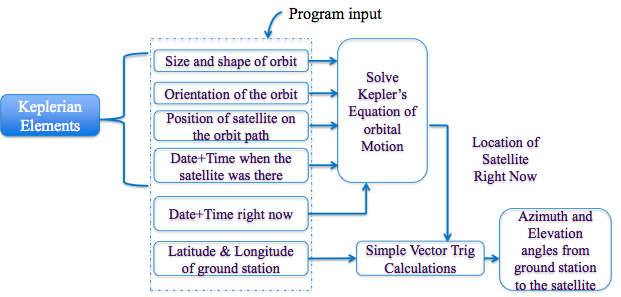
\includegraphics[width=0.9\textwidth]{images/casestudysw.png}
\end{center}

And, for reference (note that ``Zenit'' = Zenith, ``Azimut'' = Azimuth, ``Orizzonte'' = Horizon, and ``Cel. meridian'' = Celestial Meridian).

\begin{center}
	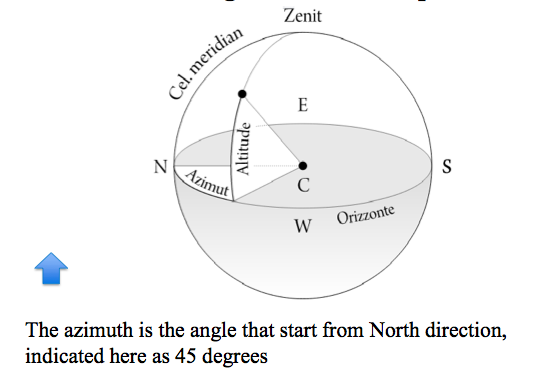
\includegraphics[width=0.75\textwidth]{images/azimuth.png}
\end{center}

Here are some problems the CSA has with the current software:

\begin{itemize}
	\item The code was outdated and did not reflect the latest changes
	\item The source code was unavailable
	\item The library was a licensed product, causing recurrent license fees
	\item The code did not respond well when being called by multiple programs
\end{itemize}

{\sf Exercise: identify some functional requirements, non-functional requirements, and constraints of this system.}

\vspace{20em}


\section*{Specifications}
After gathering your data, refining them, and using your engineering judgement to produce the software requirements, the next step is creating a specification. The specification is based on the requirements, and explains in detail how the software will meet the goals set by the requirements. Or, to put it more simply, creating the specification makes you sit down and design the program.

\section*{Motivation}

\begin{quote}
	\textit{... specs are like flossing: everybody knows they should be writing them, but nobody does.}
\end{quote}
\hfill Joel Spolsky 


There is a great temptation to just jump in to the coding and not bother ``wasting time'' on a specification. That's a very bad idea. Specifications are important and worth doing, because it is much, much faster to change the text of the spec than to rewrite or replace a piece of code. No matter how fast you are at developing software, changing the text ``file uploads take place synchronously and block the UI'' to ``file uploads take place asynchronously and do not block the UI'' takes a tiny fraction of the time it would take to make those changes in the software. Programmers also tend to get attached to code they've already written (it is psychologically difficult to throw away a piece of code just finished), so incorrect or inefficient code will remain.

The other major function of the specification is that it is a form of communication between many different parties (not just developers). Developers will have a clear idea of not just what is to be done, but also how it should be done. The spec is useful to other areas of the company as well: it can be used by QA to develop tests, by marketing, by business people, by technical writers, and by customers to make sure they are getting a product that meets their needs. Without a formal spec, there will be lots of e-mails and meetings and so on while people try to figure things out. With a spec, the information is centrally available and there is much less chance of an error \cite{spolsky:fs1}.

One final reason for creating a specification is it will be possible to make a schedule. Having designed the software in detail, you will have a good basis for the schedule. We'll discuss scheduling and planning in another upcoming lecture.

\section*{Writing a Specification}

When writing a functional specification, the goal is to describe how the product works from a user perspective: features, menus, dialogs, user interfaces, etc. The document will never be complete and perfect, but that's okay -- update it as needed.

To start with, examine the requirements you have gathered (see the previous lecture). The results of that process will be the starting point for the functional specification. When the specification is finished, it should be possible to examine each requirement and identify which sections of the specification fulfill that requirement. (Later on, during software testing and verification, it will be possible to trace the requirements from the requirements document, through the design documents, and into the verification results. Tracing requirements ensures that all requirements are met, and will make it easier to demonstrate to the customers, management, etc that this is the case.)


Designing the system should be user-focused. Consider the workflow of a user and use that to create a scenario. For example, if we're still working with the software to enter student grades, create a scenario for how a professor might want to enter them: the professor first prepares the grades, then logs into the system, navigates to the grade entry screen, selects the class, and then enters the grades next to each student number. More detail and realism in the scenario will result in a better specification \cite{spolsky:fs2}.

The most important element of the specification are the details: a description for what is going to happen in every situation... whether things go right or wrong. In fact, you will possibly spend more time describing what is supposed to happen for errors.  Imagine you are making a print button in the program. It is necessary to decide what happens in each of the following situations: 

\begin{enumerate}
	\item No printers are configured.
	\item Multiple printers are configured, but no default is set.
	\item The data is in colour but the default printer can only print black and white.
	\item The print processor encountered an error.
	\item The print job was sent, but the printer is out of paper or ink.
	\item The printer memory is insufficient to handle the print job.
	\item The print job was sent and is now in the print queue.
	\item The print job completed successfully.
\end{enumerate}

This is not an exhaustive list. The correct response to each situation depends on the system in question, but the specification should have an answer for each. Sometimes, that answer might be ``nothing happens'', and that's fine; document, however, that nothing happening is the expected behaviour.

If you encounter a situation where there is no specification describing what should happen, this should be addressed. Your judgement may tell you what the correct solution is, but you should nevertheless update the specification.

\paragraph{A Collection of Stories.} If this seems familiar, it's because it should. In the previous lecture we talked about stories, and a specification can be simply a collection of stories. If you are using Behaviour Driven Development, or at least the idea of stories, a specification is created as you create the requirements. The specification is done once all the stories are written and assembled. Easy!

Update the specification regularly. If it's never updated, it will soon fall out of date and become useless if not actively misleading. Much like cleaning a home, if you do a little bit every day the amount of work seems manageable; if you ignore it for a long time then it becomes a full day of work.

Writing a specification as a team effort is usually painful. If the scope of the software is too large for a single person to write the specification, it should be divided into sections and one person should be responsible for each section. If it is being split up, it's important to co-ordinate to keep things consistent between the different modules \cite{spolsky:fs2}.


\paragraph{Write simply} There's no need for a specification (formal or otherwise) to be full of big, long words and complicated sentences. Writing ``utilize'' instead of ``use'' doesn't make the specification any better or clearer. Turning a simple sentence like ``the query must complete within 10 seconds'' into ``It is an absolute requirement that under all circumstances that should a user elect to execute a query on the system, the maximum upper bound on execution time thereof is 10 seconds'' is actively making the specification worse. Simpler and easier to understand is better. Using long words and fancy, complicated sentences do not make the document more professional, either \cite{spolsky:fs4}:


\section*{Example}
We will now take some excerpts from the specification for \textit{Fog Creek Copilot}, a piece of software for providing technical support over the internet (``Hello, IT, have you tried turning it off and on again?'')~\cite{copilotspec}. The product was referred to in its internal pre-release documentation as ``Aardvark''. The excerpts will provide some examples of key components in the spec and how they might look. 


\paragraph{Overview.} The specification starts with a general overview of what the software is supposed to do: ``Aardvark allows people to help their friends, relatives, and customers with their computer problems by temporarily taking over their computers over the Internet.'' This included a more detailed description of what the product is supposed to do from a user point of view.

\paragraph{Major Features.} The overview is followed immediately by a list of features:
\begin{itemize}
	\item Easy to get started: \begin{itemize} \item No software needs to be permanently installed; \item Simple fast payment and no commitment \end{itemize}
	\item Version 1.0 is Windows only and requires a reasonable broadband connection.
	\item Blasts through all firewalls as long as outbound connections on port 443 are allowed.
	\item Secure (hopefully).
\end{itemize}

The list of major features is really quite simple and describes well enough what the software does. Perfect detail is not necessary, but this explains for developers, marketing, and all other parties.

\paragraph{Making Changes Early.}
Changing the specification is a lot easier than changing things once underway:

\begin{quote}
\textit{When I wrote the first draft of this spec, I had a more complicated flowchart that assumed that either party (helper or victim) could initiate the process. This became extremely complicated and convoluted for various reasons. As I worked through the screens that would be needed to allow either party to initiate the process, I realized that Aardvark would be just as useful, and radically simpler, if the helper was required to start the whole process. Making this change in the spec took an hour or two. If we had made this change in code, it would have added weeks to the schedule.}
\end{quote}

\paragraph{UI Examples.}
The specification also has a bunch of UI examples. The art quality is not very good, but it explains in simple terms what things should look like:

\begin{center}
	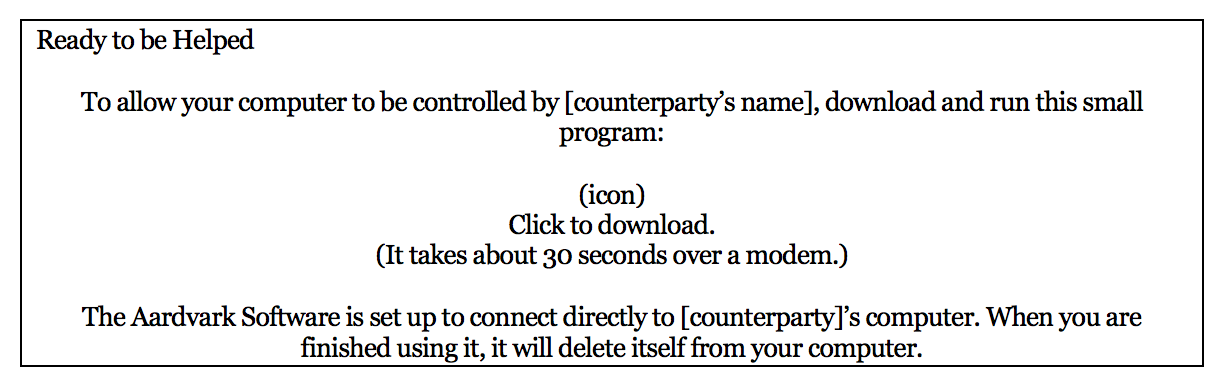
\includegraphics[width=0.75\textwidth]{images/aardvarkui.png}
\end{center}

\paragraph{Future Features.}
Future features are valuable both as a list of things to do in the future, and as a list of things \textit{not} to do in the current version. Some examples:

\begin{itemize}
	\item Ability to transfer files between helper and victim, possibly with drag and drop.
	\item Chat features, either voice or IM style.
\end{itemize}

\paragraph{Pictures are Worth a Thousand Words.}
The saying that a picture is worth a thousand words is often literally true in a specification. Use graphics where appropriate. See the following example from the Aardvark spec, describing a workflow. If this were written out using text it would be several pages of complicated text.

\begin{center}
	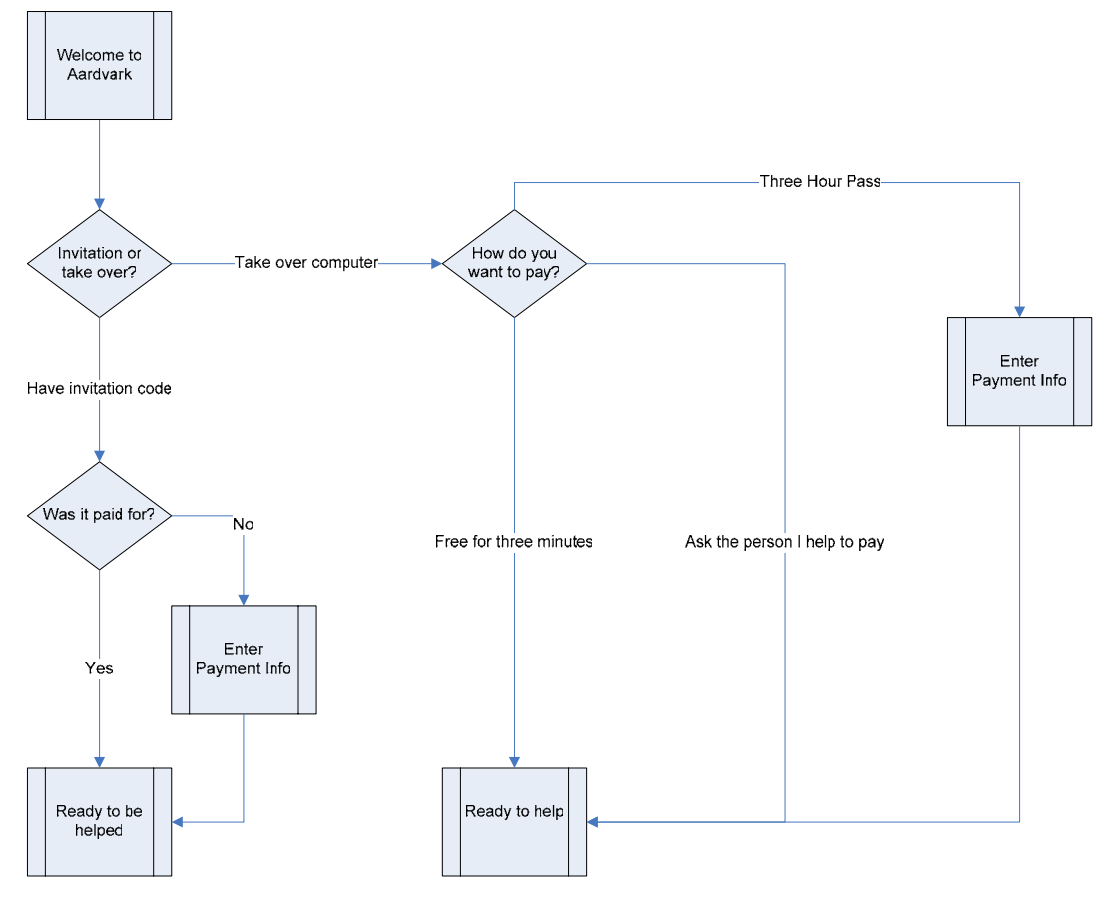
\includegraphics[width=0.75\textwidth]{images/aardvarksite.png}
\end{center}



\bibliographystyle{alpha}
\bibliography{155}


\end{document}